\documentclass[english,serif,mathserif,xcolor=pdftex,dvipsnames,table]{beamer}
\usetheme[informal]{gc3}
\usepackage{gc3}

\title[OOP 1]{%
  Object-orientation, I
}
\author[GC3]{%
  GC3: Grid Computing Competence Center, \\
  University of Zurich
}
\date{Mar.~19--20, 2014}

\begin{document}

% title frame
\maketitle


\begin{frame}
  \frametitle{What we shall see in this part}

  How to define custom Python objects.

  \+
  We shall use \href{http://jccc-mpg.wikidot.com/vectors}{2D
    vectors} as examples.
\end{frame}


\begin{frame}
  \frametitle{Recall: \emph{What is an object}?}
  \textbf{A Python object is a bundle of variables and functions.}

  \+
  What variable names and functions comprise an object is defined
  by the object's \emph{class}.

  \+
  From one class specification, many objects can be
  \emph{instanciated}.  Different instances can assign different
  values to the object variables.

  \+
  Variables and functions in an instance are collectively called
  \emph{instance attributes}; functions are also termed \emph{instance
    methods}.
\end{frame}


\begin{frame}
  \frametitle{Recall: \emph{What is a 2D vector?}}

  A \emph{2D} vector is an element of the vector space
  $\mathbb{R}^2$.

  \+
  Every \emph{2D} vector $\mathbf{u}$ is completely described by a
  pair of real coordinates $\langle u_x, u_y \rangle$.
  Two operations are defined on vectors:

  \+
  \begin{columns}
    \begin{column}{0.6\linewidth}
      \raggedleft
      \emph{vector addition:} if $\mathbf{w} = \mathbf{u} +
        \mathbf{v}$, then $w_x = u_x + v_x$ and $w_y = u_y + v_y$.
    \end{column}
    \begin{column}{0.4\linewidth}
      \centering
      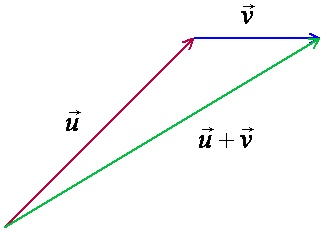
\includegraphics[height=4\baselineskip]{fig/VectorAddition.jpg}
    \end{column}
  \end{columns}

  \+
  \begin{columns}
    \begin{column}{0.4\linewidth}
      \centering
      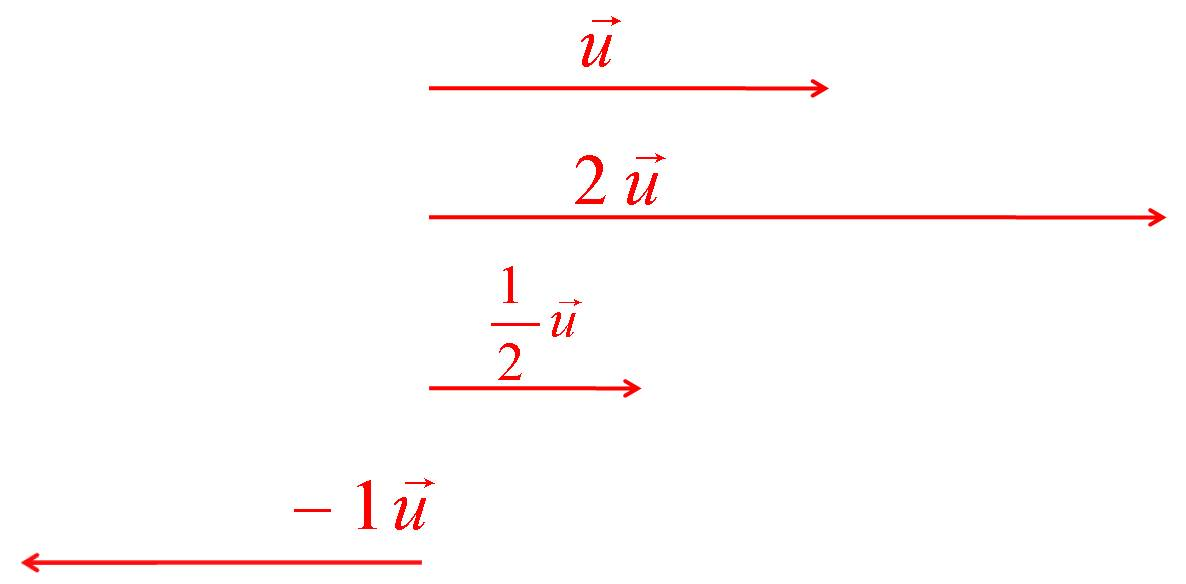
\includegraphics[height=3\baselineskip]{fig/VectorScalarMultiplication.jpg}
    \end{column}
    \begin{column}{0.6\linewidth}
      \raggedright
      \emph{scalar multiplication:} if $\mathbf{v} = \alpha
      \cdot \mathbf{u}$ with $\alpha \in \mathbb{R}$, then $v_x =
      \alpha \cdot u_x$ and $v_y = \alpha \cdot u_y$.
    \end{column}
  \end{columns}

  \begin{references}
    \tiny
    Images courtesy of \url{http://jccc-mpg.wikidot.com/vectors},
    which see for precise definitions and discussion of 2D vectors.
  \end{references}
\end{frame}


\begin{frame}[fragile]
  \frametitle{A \emph{2D vector} in Python}
  \begin{columns}[t]
    \begin{column}{0.5\textwidth}
\begin{lstlisting}
class Vector(object):
  """A 2D Vector."""
  def __init__(self, x, y):
    self.x = x
    self.y = y
  def add(self, other):
    return Vector(self.x+other.x,
                  self.y+other.y)
  def mul(self, scalar):
    return Vector(scalar*self.x, scalar*self.y)
  def show(self):
    return ("<%g,%g>" % (self.x, self.y))
\end{lstlisting}
    \end{column}
    \begin{column}{0.5\textwidth}
      \raggedleft
      This code defines a Python object that implements a 2D vector.
    \end{column}
  \end{columns}

  \+
  {\scriptsize Source code available at:
    \url{https://raw.github.com/gc3-uzh-ch/python-course/master/vector.py}}
\end{frame}


\begin{frame}[fragile]
  \frametitle{What does \texttt{Vector} do?}
  \begin{columns}
    \begin{column}[t]{0.5\linewidth}
  We can create vectors by initializing them with the two coordinates
  $(x,y)$:
\begin{lstlisting}
>>> u = Vector(1,0)
>>> v = Vector(0,1)
\end{lstlisting}
    \end{column}
    \begin{column}[t]{0.5\linewidth}
      The \texttt{show} method shows vector coordinates:
\begin{lstlisting}
>>> u.show()
'<1,0>'
>>> v.show()
'<0,1>'
\end{lstlisting}
    \end{column}
  \end{columns}

  \+
  \begin{columns}
    \begin{column}[t]{0.5\linewidth}
      The \texttt{add} method implements vector addition:
\begin{lstlisting}
>>> w = u.add(v)
>>> w.show()
'<1,1>'
\end{lstlisting}
    \end{column}
    \begin{column}[t]{0.5\linewidth}
      The \texttt{mul} method implements scalar multiplication:
\begin{lstlisting}
>>> v2 = v.mul(2)
>>> v2.show()
'<0,2>'
\end{lstlisting}
    \end{column}
  \end{columns}
\end{frame}


\begin{frame}[fragile]
  \frametitle{User-defined classes, I}
  \begin{columns}[t]
    \begin{column}{0.5\textwidth}
\begin{lstlisting}
~\HL{class}~ Vector(object):
  """A 2D Vector."""
  def __init__(self, x, y):
    self.x = x
    self.y = y
  def add(self, other):
    return Vector(self.x+other.x,
                  self.y+other.y)
  def mul(self, scalar):
    return Vector(scalar*self.x, scalar*self.y)
  def show(self):
    return ("<%g,%g>" % (self.x, self.y))
\end{lstlisting}
    \end{column}
    \begin{column}{0.5\textwidth}
      \raggedleft
      A class definition starts with the keyword \texttt{class}.

      The class definition is indented relative to the \texttt{class}
      statement.
    \end{column}
  \end{columns}
\end{frame}


\begin{frame}[fragile]
  \frametitle{User-defined classes, II}
  \begin{columns}[t]
    \begin{column}{0.5\textwidth}
\begin{lstlisting}
class Vector~\HL{(object)}~:
  """A 2D Vector."""
  def __init__(self, x, y):
    self.x = x
    self.y = y
  def add(self, other):
    return Vector(self.x+other.x,
                  self.y+other.y)
  def mul(self, scalar):
    return Vector(scalar*self.x, scalar*self.y)
  def show(self):
    return ("<%g,%g>" % (self.x, self.y))
\end{lstlisting}
    \end{column}
    \begin{column}{0.5\textwidth}
      \raggedleft
      This identifies user-defined~classes.

      \+
      (Do not leave it out or you'll get an ``old-style'' class, which
      is deprecated behavior.)
    \end{column}
  \end{columns}
\end{frame}


\begin{frame}[fragile]
  \frametitle{User-defined classes, II}
  \begin{columns}[t]
    \begin{column}{0.5\textwidth}
\begin{lstlisting}
class Vector(object):
  ~\HL{"""A 2D Vector."""}~
  def __init__(self, x, y):
    self.x = x
    self.y = y
  def add(self, other):
    return Vector(self.x+other.x,
                  self.y+other.y)
  def mul(self, scalar):
    return Vector(scalar*self.x, scalar*self.y)
  def show(self):
    return ("<%g,%g>" % (self.x, self.y))
\end{lstlisting}
    \end{column}
    \begin{column}{0.5\textwidth}
      \raggedleft
      Classes can have docstrings.

      The content of a class docstring will be shown as help text for
      that class.
    \end{column}
  \end{columns}
\end{frame}


\begin{frame}[fragile]
  \frametitle{User-defined classes, IV}
  \begin{columns}[t]
    \begin{column}{0.5\textwidth}
\begin{lstlisting}
class Vector(object):
  """A 2D Vector."""
  ~\HL{\textbf{def} \_\_init\_\_(\textbf{self}, x, y):}~
    self.x = x
    self.y = y
  def add(self, other):
    return Vector(self.x+other.x,
                  self.y+other.y)
  def mul(self, scalar):
    return Vector(scalar*self.x, scalar*self.y)
  def show(self):
    return ("<%g,%g>" % (self.x, self.y))
\end{lstlisting}
    \end{column}
    \begin{column}{0.5\textwidth}
      \raggedleft
      The {\bf def} keyword introduces a method~definition.

      \+
      Every method \emph{must} have at~least one argument,
      named~{\bf self}.
    \end{column}
  \end{columns}
\end{frame}


\begin{frame}[fragile]
  \frametitle{The \texttt{self} argument}

  \textbf{Every method of a Python object always has \texttt{self}
    as first argument.}

  \+
  However, you do not specify it when calling a method: it's
  automatically inserted by Python:
\begin{lstlisting}
>>> class ShowSelf(object):
...   def show(self):
...     print(self)
...
>>> x = ShowSelf() # construct instance
>>> x.show() # `self' automatically inserted!
<__main__.ShowSelf object at 0x299e150>
\end{lstlisting}

  \+
  The \texttt{self} name is a reference to the object instance
  itself.  You \emph{need to} use \texttt{self} when accessing methods
  or attributes of this instance.
\end{frame}


\begin{frame}
  \frametitle{No access control}
  There are no ``public''/``private''/etc. qualifiers for object
  attributes.

  \+
  \textbf{\emph{Any} code can create/read/overwrite/delete \emph{any} attribute on
    \emph{any} object.}

  \+
  There are \emph{conventions}, though:
  \begin{itemize}
  \item ``protected'' attributes: \texttt{\_name}
  \item ``private'' attributes: \texttt{\_\_name}
  \end{itemize}
  (But again, note that this is not \emph{enforced} by the system in
  any way.)

\end{frame}


\begin{frame}[fragile]
  \frametitle{Name resolution rules, I}
  \small

  Within a function body, names are resolved according to \href{http://stackoverflow.com/questions/291978/short-description-of-python-scoping-rules/292502#292502}{the LEGB rule}:
  \begin{description}
  \item[L] Local scope: any names defined in the current function;
  \item[E] Enclosing function scope: names defined in enclosing
    functions (outermost last);
  \item[G] global scope: names defined in the toplevel of the enclosing module;
  \item[B] Built-in names (i.e., Python's \texttt{\_\_builtins\_\_} module).
  \end{description}

  \+
  \textbf{Any name that is not in one of the above scopes \emph{must}
    be qualified.}

  \+
  So you have to write \texttt{self.x} to reference an attribute in
  this instance, \texttt{datetime.date} to mean a class defined in module
  \texttt{date}, etc.

  % \begin{references}
  %   \url{http://stackoverflow.com/questions/291978/short-description-of-python-scoping-rules/292502#292502}
  % \end{references}
\end{frame}


\begin{frame}[fragile]
  \frametitle{Name resolution rules, II}
  \begin{columns}
    \begin{column}[t]{0.6\linewidth}
\begin{lstlisting}
import datetime as dt

def today():
  ~\HL{td}~ = dt.date.today()
  return "today is " + ~\HL{td}~.isoformat()

def hey(~\HL{name}~):
  print("Hey " + ~\HL{name}~ + "; " + today())

hey("you")
\end{lstlisting}
    \end{column}
    \begin{column}[t]{0.4\linewidth}
      \raggedleft
      Unqualified name within a function: resolves to a local variable.
    \end{column}
  \end{columns}
\end{frame}


\begin{frame}[fragile]
  \frametitle{Name resolution rules, III}
  \begin{columns}
    \begin{column}[t]{0.6\linewidth}
\begin{lstlisting}
import datetime as dt

def today():
  td = dt.date.today()
  return "today is " + td.isoformat()

def hey(name):
  print("Hey " + name + "; " + ~\HL{today}~())

hey("you")
\end{lstlisting}
    \end{column}
    \begin{column}[t]{0.4\linewidth}
      \raggedleft
      Unqualified name: since there is no local variable by that name,
      it resolves to a module-level binding, i.e., to the
      \texttt{today} function defined above.
    \end{column}
  \end{columns}
\end{frame}


\begin{frame}[fragile]
  \frametitle{Name resolution rules, IV}
  \begin{columns}
    \begin{column}[t]{0.6\linewidth}
\begin{lstlisting}
import datetime as ~\HL[Red!25]{dt}~

def today():
  td = ~\HL{dt}~.date.today()
  return "today is " + td.isoformat()

def hey(name):
  print("Hey " + name + "; " + today())

hey("you")
\end{lstlisting}
    \end{column}
    \begin{column}[t]{0.4\linewidth}
      \raggedleft
      Unqualified name: resolves to the \texttt{dt} name created at global scope by the \texttt{import} statement.
    \end{column}
  \end{columns}
\end{frame}


\begin{frame}[fragile]
  \frametitle{Name resolution rules, V}
  \begin{columns}
    \begin{column}[t]{0.6\linewidth}
\begin{lstlisting}
import datetime as dt

def today():
  td = ~\HL{dt.date}~.today()
  return "today is " + td.isoformat()

def hey(name):
  print("Hey " + name + "; " + today())

hey("you")
\end{lstlisting}
    \end{column}
    \begin{column}[t]{0.4\linewidth}
      \raggedleft
      Qualified name: instructs Python to search the
      \texttt{date} attribute within the \texttt{dt} module.
    \end{column}
  \end{columns}
\end{frame}


\begin{frame}[fragile]
  \frametitle{Name resolution rules, VI}
  \begin{columns}
    \begin{column}[t]{0.6\linewidth}
\begin{lstlisting}
import datetime as dt

def today():
  td = dt.date.today()
  return "today is " + ~\HL{td.isoformat}~()

def hey(name):
  print("Hey " + name + "; " + today())

hey("you")
\end{lstlisting}
    \end{column}
    \begin{column}[t]{0.4\linewidth}
      \raggedleft
      Qualified name: Python searches the \texttt{isoformat} attribute
      within the \texttt{td} object instance.
    \end{column}
  \end{columns}
\end{frame}


\begin{frame}[fragile]
  \frametitle{Name resolution rules, VI}
  \begin{columns}
    \begin{column}[t]{0.6\linewidth}
\begin{lstlisting}
class Vector(object):
  def __init__(self, ~\HL[Red!25]{x}~, ~\HL[Red!25]{y}~):
    self.x = ~\HL{x}~
    self.y = ~\HL{y}~
  # ...
\end{lstlisting}
    \end{column}
    \begin{column}[t]{0.4\linewidth}
      \raggedleft
      Unqualified name: resolves to a local variable in
      scope of function \lstinline|__init__|.
    \end{column}
  \end{columns}
\end{frame}


\begin{frame}[fragile]
  \frametitle{Name resolution rules, VII}
  \begin{columns}
    \begin{column}[t]{0.6\linewidth}
\begin{lstlisting}
class Vector(object):
  def __init__(self, x, y):
    ~\HL{self.x}~ = x
    ~\HL{self.y}~ = y
  # ...
\end{lstlisting}
    \end{column}
    \begin{column}[t]{0.4\linewidth}
      \raggedleft
      Qualified names: resolve to attributes in object \lstinline|self|.

      \+ (Actually, \lstinline|self.x = ...| \emph{creates} the
      attribute \lstinline|x| on \lstinline|self| if it does not exist
      yet.)
    \end{column}
  \end{columns}

\end{frame}


\begin{frame}[fragile]
  \frametitle{Object initialization}
  \begin{columns}[t]
    \begin{column}{0.5\textwidth}
\begin{lstlisting}
class Vector(object):
  """A 2D Vector."""
  ~\HL{\textbf{def} \_\_init\_\_(\textbf{self}, x, y):}~
    self.x = x
    self.y = y
  def add(self, other):
    return Vector(self.x+other.x, self.y+other.y)
  def mul(self, scalar):
    return Vector(scalar*self.x, scalar*self.y)
  def show(self):
    return ("<%g,%g>" % (self.x, self.y))
\end{lstlisting}
    \end{column}
    \begin{column}{0.5\textwidth}
      \raggedleft
      The \lstinline|__init__| method has a special
      meaning: it is called when an instance is created.
    \end{column}
  \end{columns}
\end{frame}



\begin{frame}[fragile]
  \frametitle{Constructors}

  The \lstinline|__init__| method is the object constructor.
  It should \emph{never} return any value.

  \+
  You never call \lstinline|__init__| directly, it is invoked by
  Python when a new object is created from the class:
\begin{lstlisting}
# calls Vector.\_\_init\_\_
v = Vector(0,1)
\end{lstlisting}

  \+
  The arguments to \lstinline|__init__| are the arguments you
  should supply when creating a class instance.

  \+
  (Again, minus the \texttt{self} part which is automatically
  inserted by Python.)
\end{frame}


% \begin{frame}
%   \frametitle{No overloading}

%   \textbf{Python does not allow overloading of functions.}

%   \+
%   Any function.

%   \+
%   Hence, no overloading of constructors.

%   \+
%   So: \textbf{a class has one and only one constructor.}
% \end{frame}


\begin{frame}[fragile]
  \begin{exercise}
    Add a new method \texttt{norm} the \texttt{Vector} class: if
    \texttt{v} is an instance of class \texttt{Vector}, then calling
    \texttt{v.norm()} returns the norm $\sqrt{v_x^2 + v_y^2}$ of
    the associated vector.
    (You will need the
    \href{http://docs.python.org/2/library/math.html}{math} standard
    module for computing square roots.)
  \end{exercise}

  \+
  \begin{exercise}
    Add a new method \texttt{unit} to the \texttt{Vector} class: if
    \texttt{v} is an instance of class \texttt{Vector}, then calling
    \texttt{v.unit()} returns the vector \texttt{u} having the
    same direction as \texttt{v} but norm $1$.
  \end{exercise}
\end{frame}


\end{document}

%%% Local Variables:
%%% mode: latex
%%% TeX-master: t
%%% End:
